\message{ !name(06_irf.tex)}\documentclass[../main/main.tex]{subfiles}
\begin{document}

\message{ !name(06_irf.tex) !offset(532) }



\begin{figure}[ht]
  \centering
  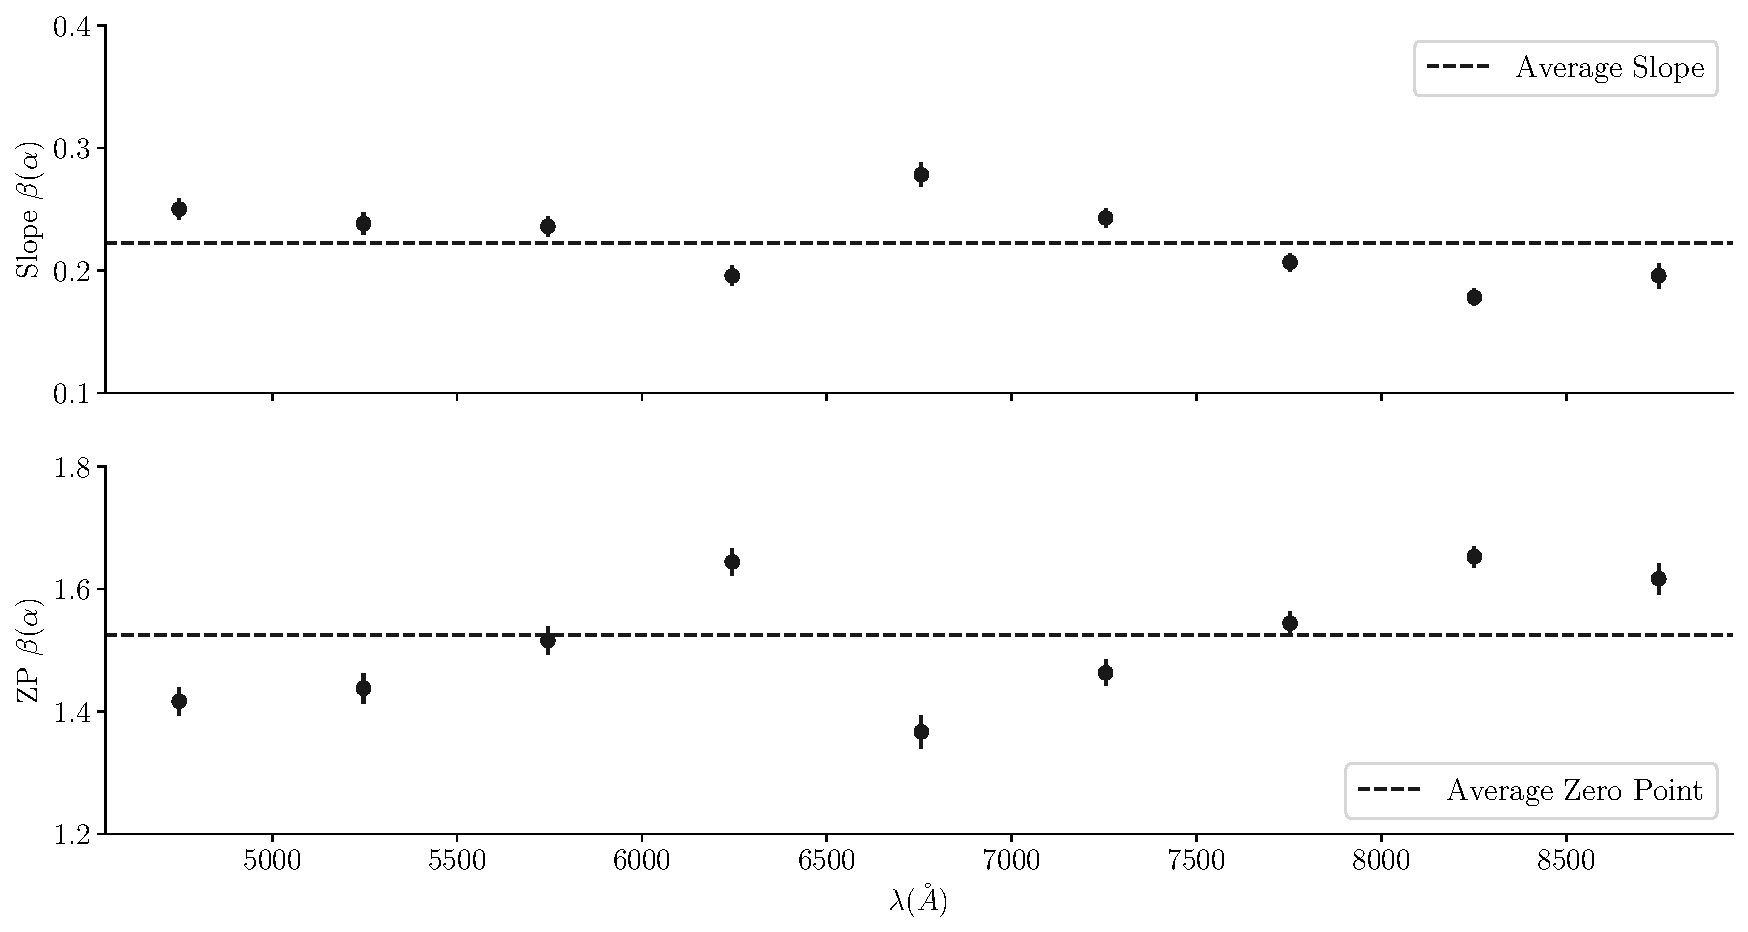
\includegraphics[width=0.8\textwidth]{../figures/06_irf/chromaticitybeta_alpha_corr.pdf}
  \caption[Chromaticité de la pente et du point zéro entre $\alpha$ et $\beta$]{Chromaticité de la pente et du point zéro entre $\alpha$ et $\beta$}
  \label{fig:chromslope_zp_alphabeta}
\end{figure}

\begin{figure}[ht]
  \centering
  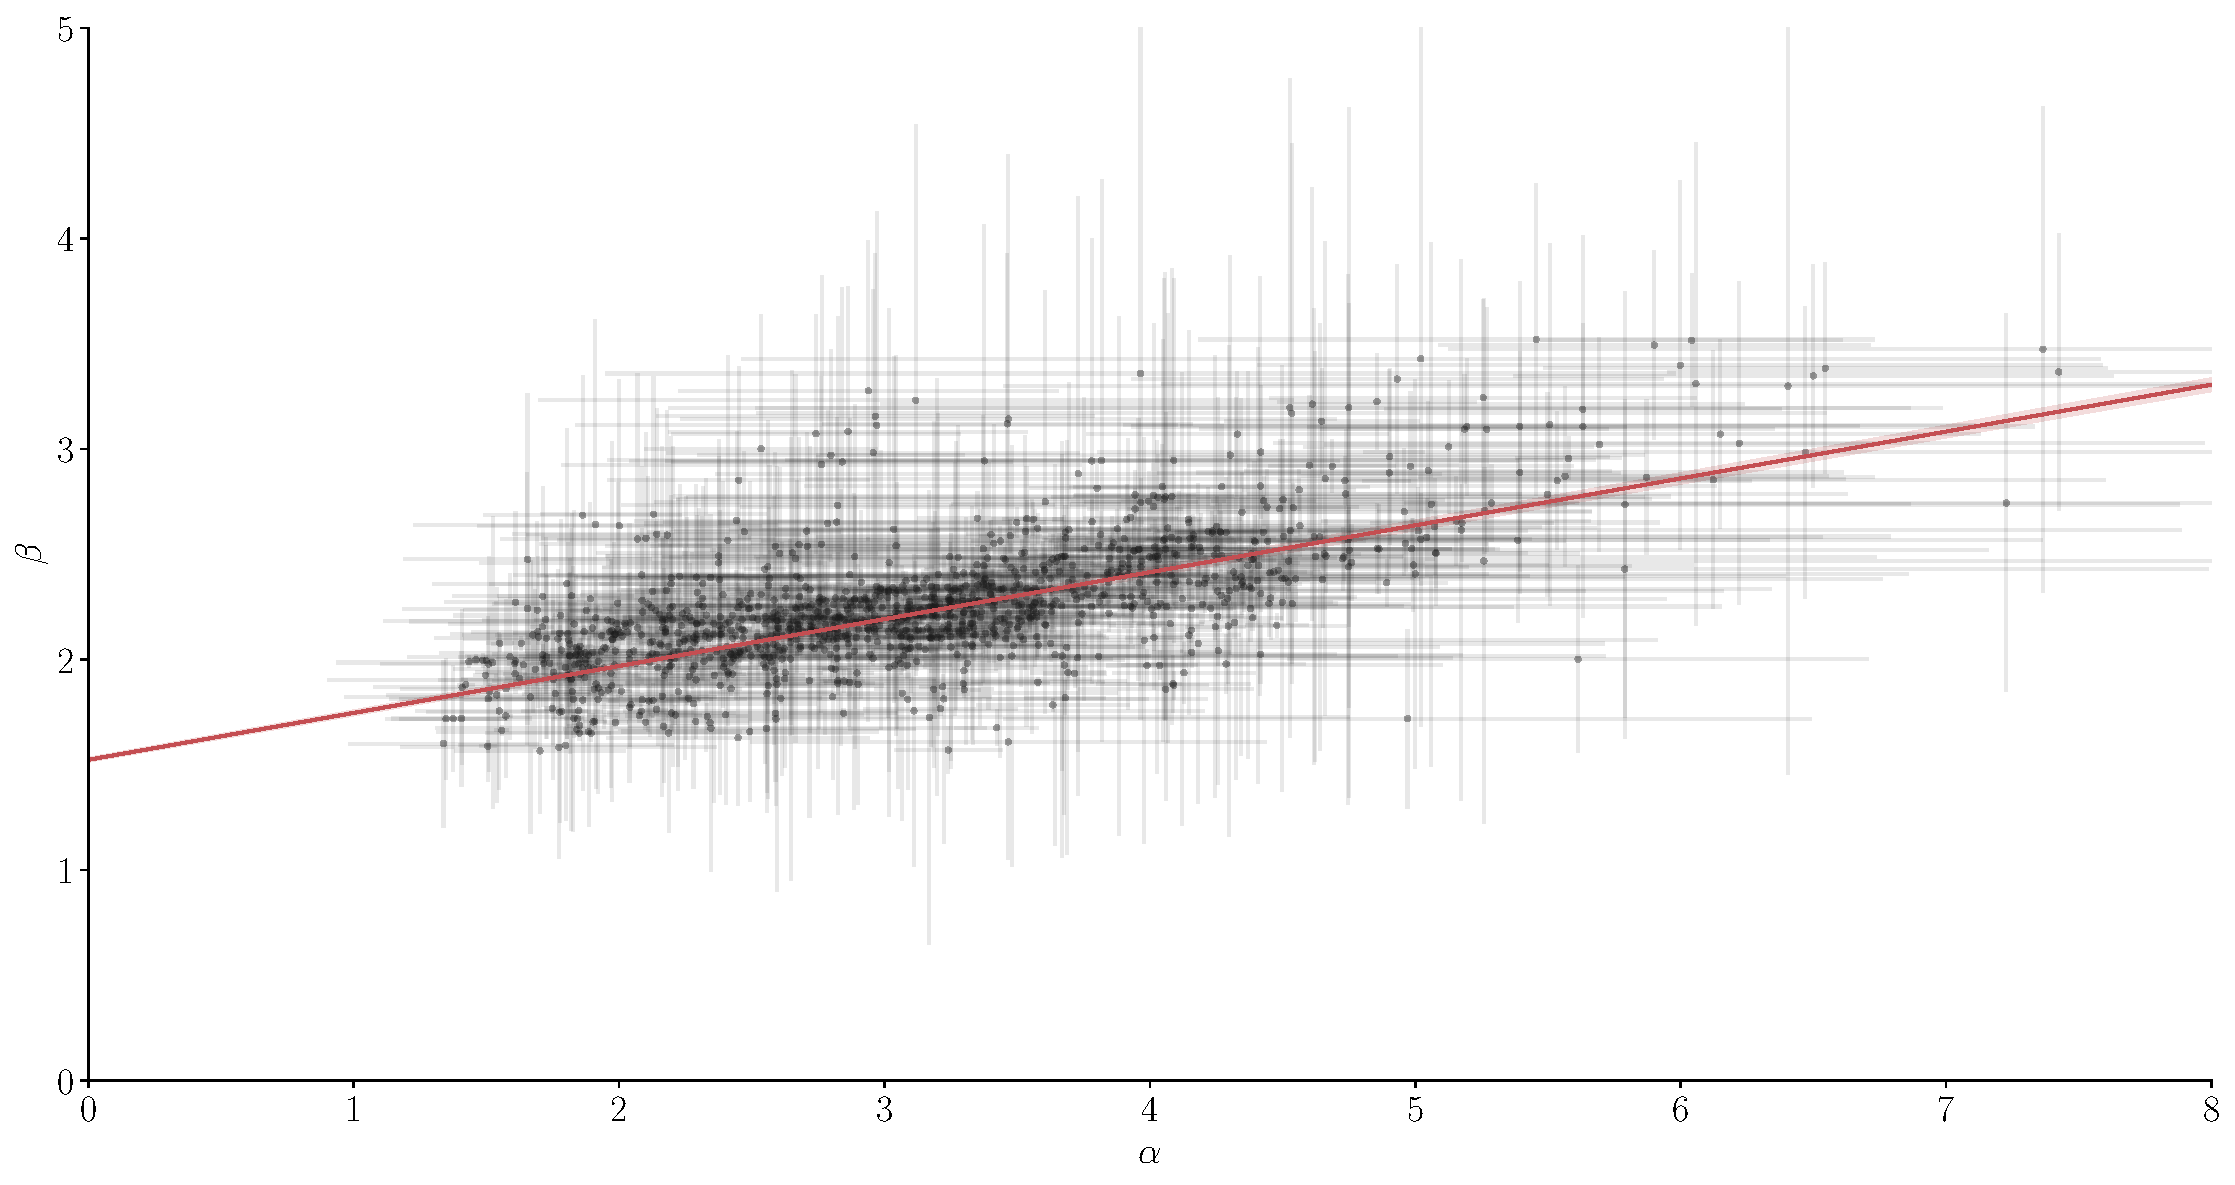
\includegraphics[width=0.8\textwidth]{../figures/06_irf/STD_alpha_beta_corr.pdf}
  \caption[]{}
  \label{fig:corralphabeta_achrom}
\end{figure}

\begin{figure}[ht]
  \centering
  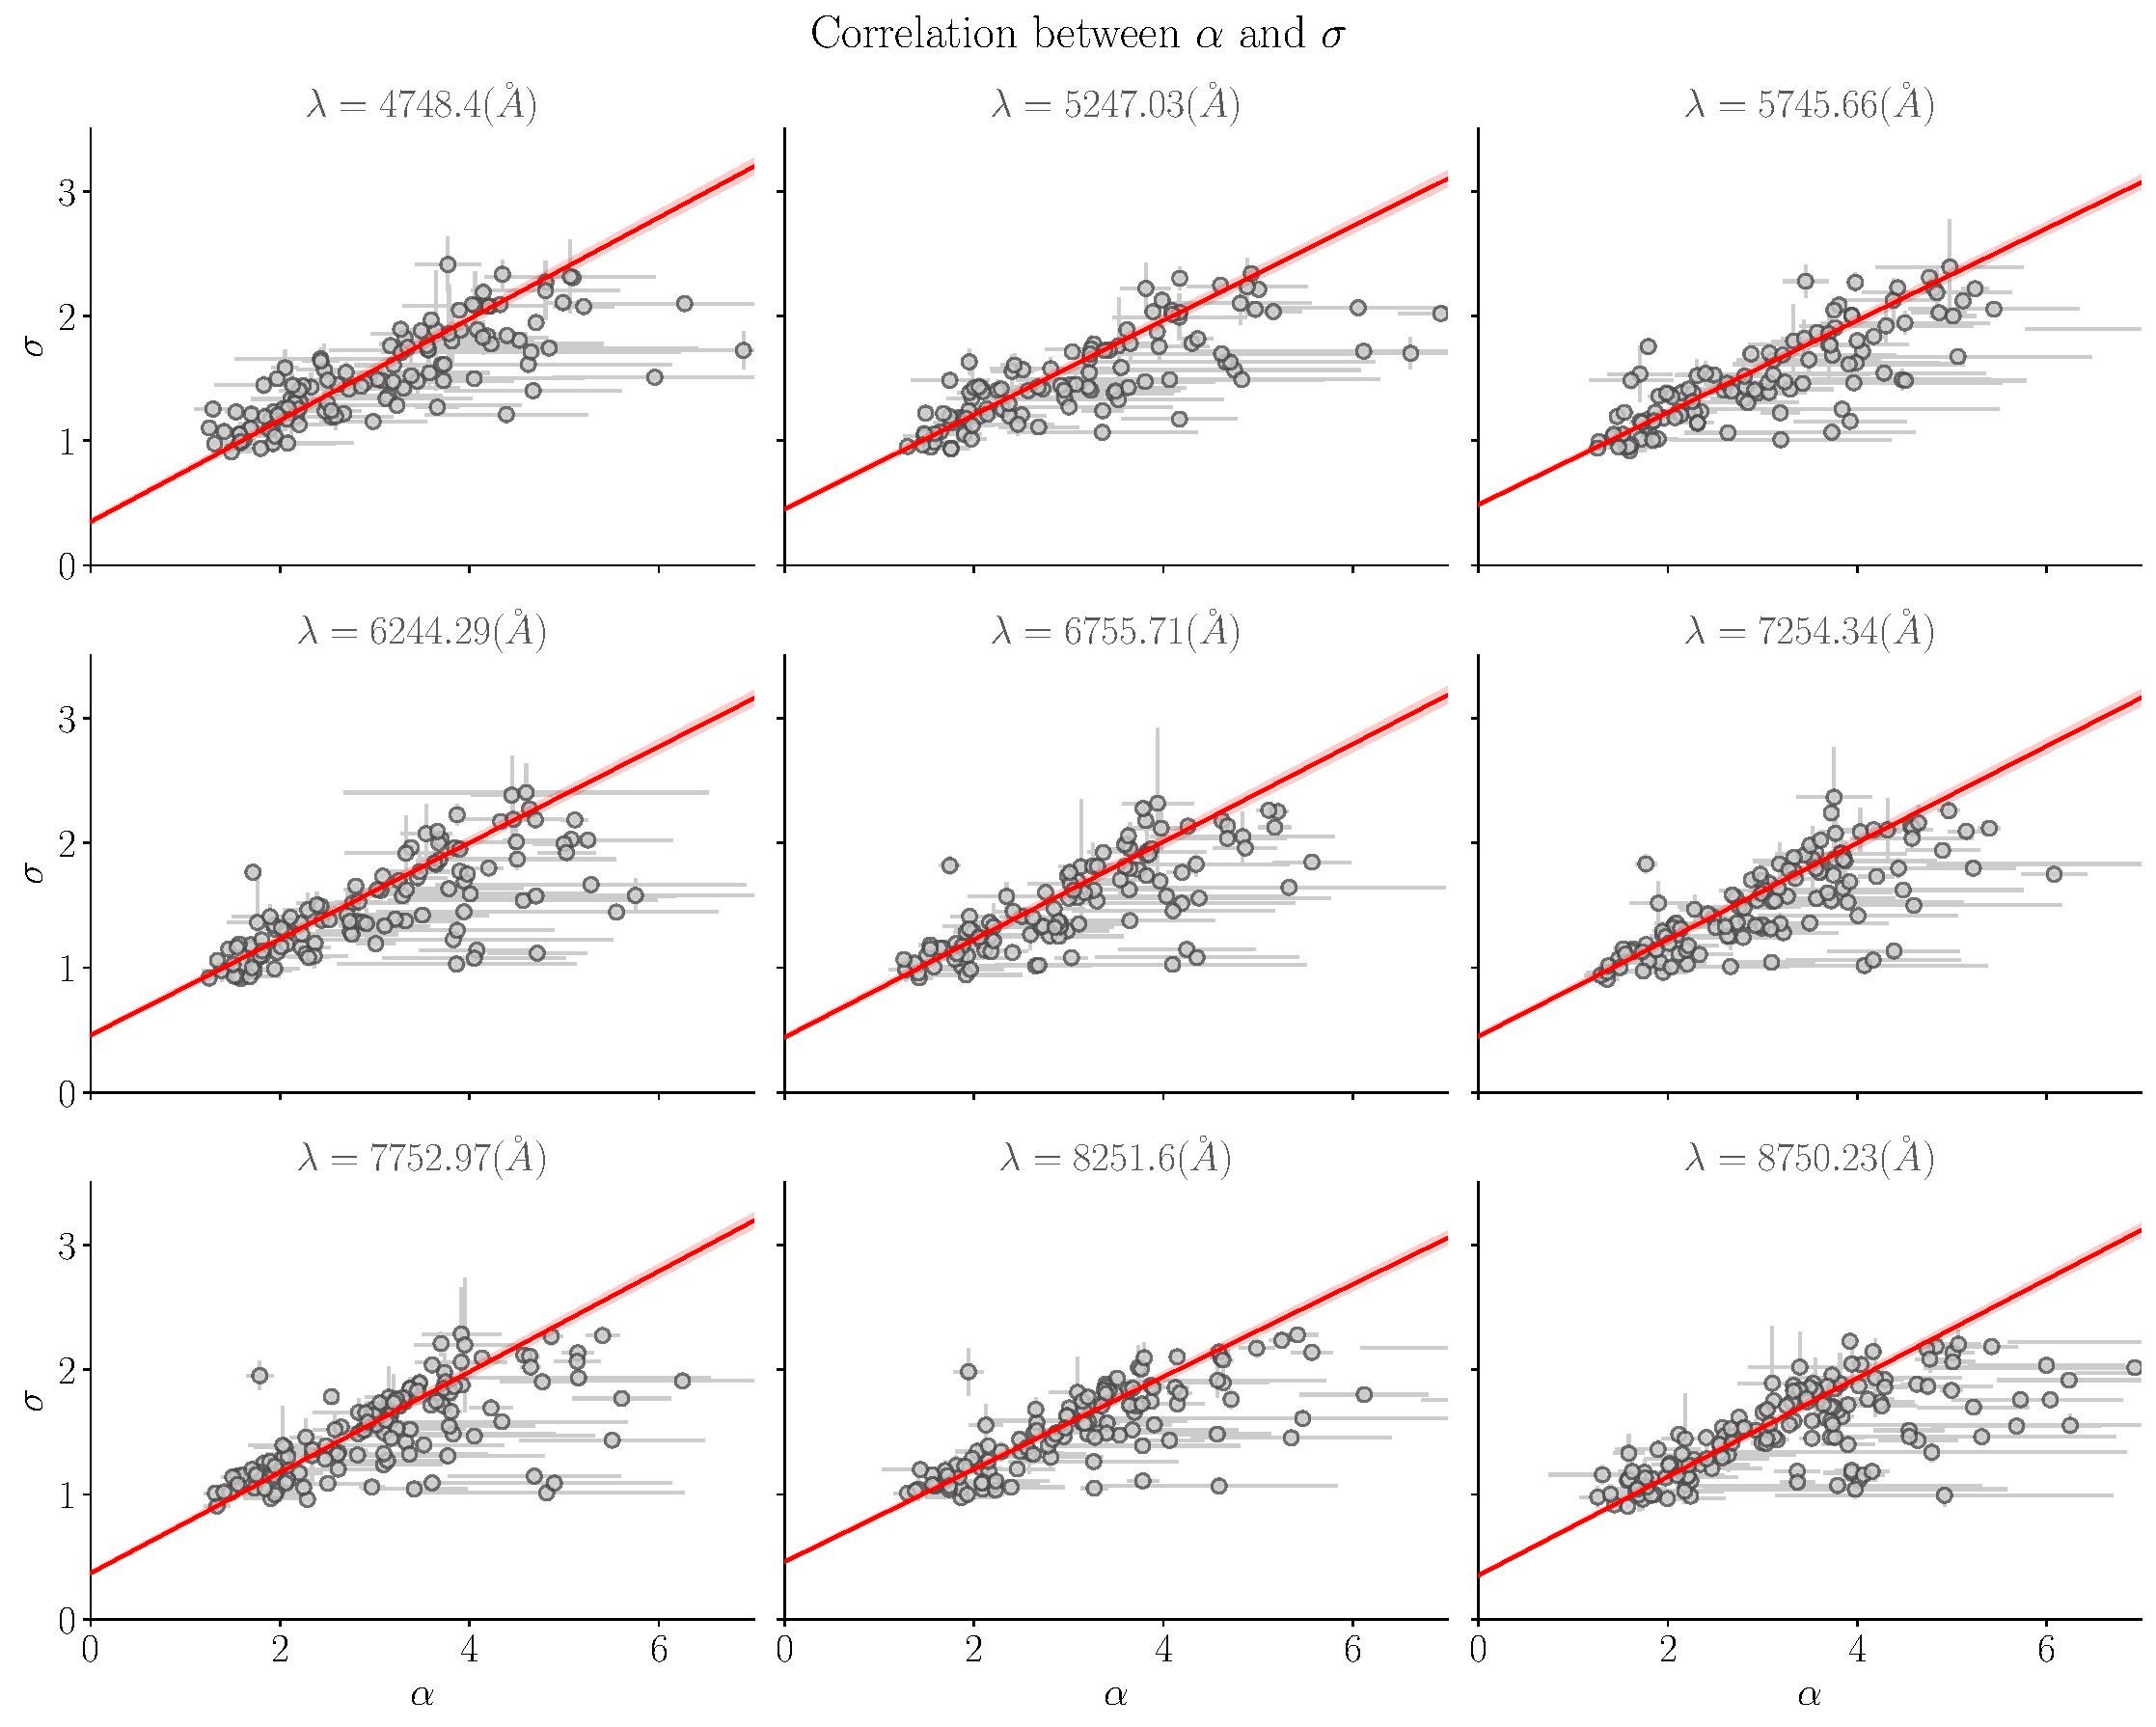
\includegraphics[width=0.9\textwidth]{../figures/06_irf/STD_alpha_sigma_chromatic_corr.pdf}
  \caption[Chromaticité des corrélations entre $\alpha$ et $\sigma$]{Chromaticité des corrélations entre $\alpha$ et $\sigma$}
  \label{fig:alphasigmachromcorr}
\end{figure}

\begin{figure}[ht]
  \centering
  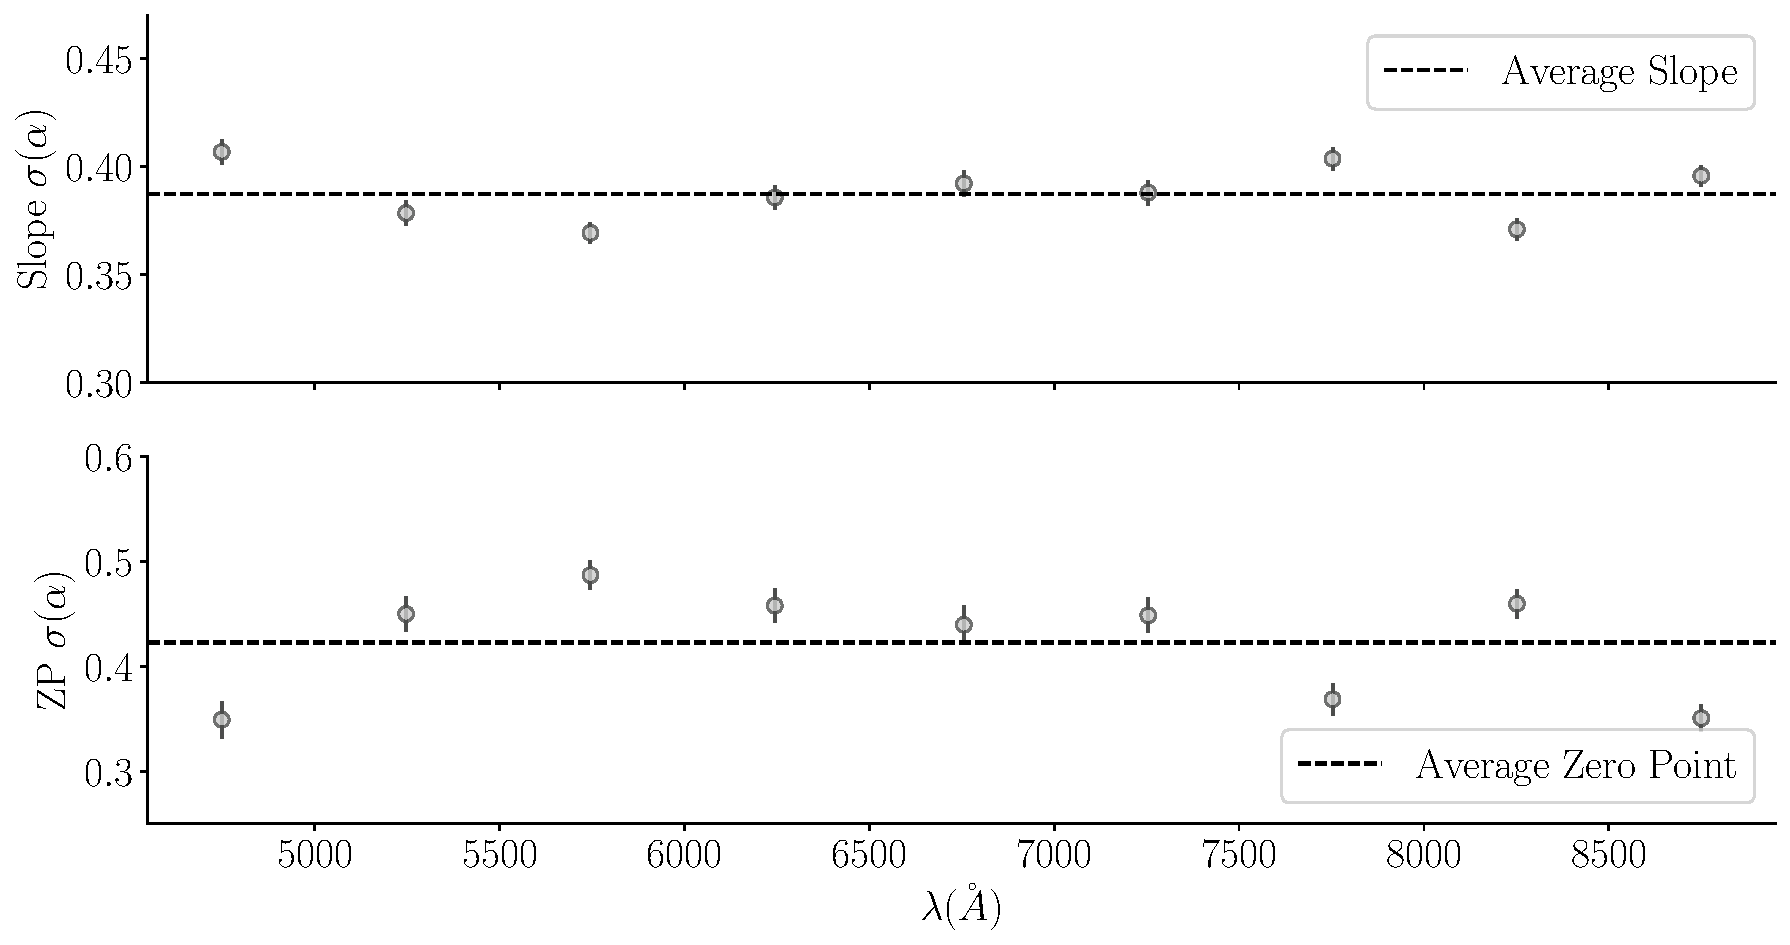
\includegraphics[width=0.8\textwidth]{../figures/06_irf/chromaticitysigma_alpha_corr.pdf}
  \caption[Chromaticité de la pente et du point zéro entre $\alpha$ et $\sigma$]{Chromaticité de la pente et du point zéro entre $\alpha$ et $\sigma$}
  \label{fig:chromslope_zp_alphasigma}
\end{figure}

\begin{figure}[ht]
  \centering
  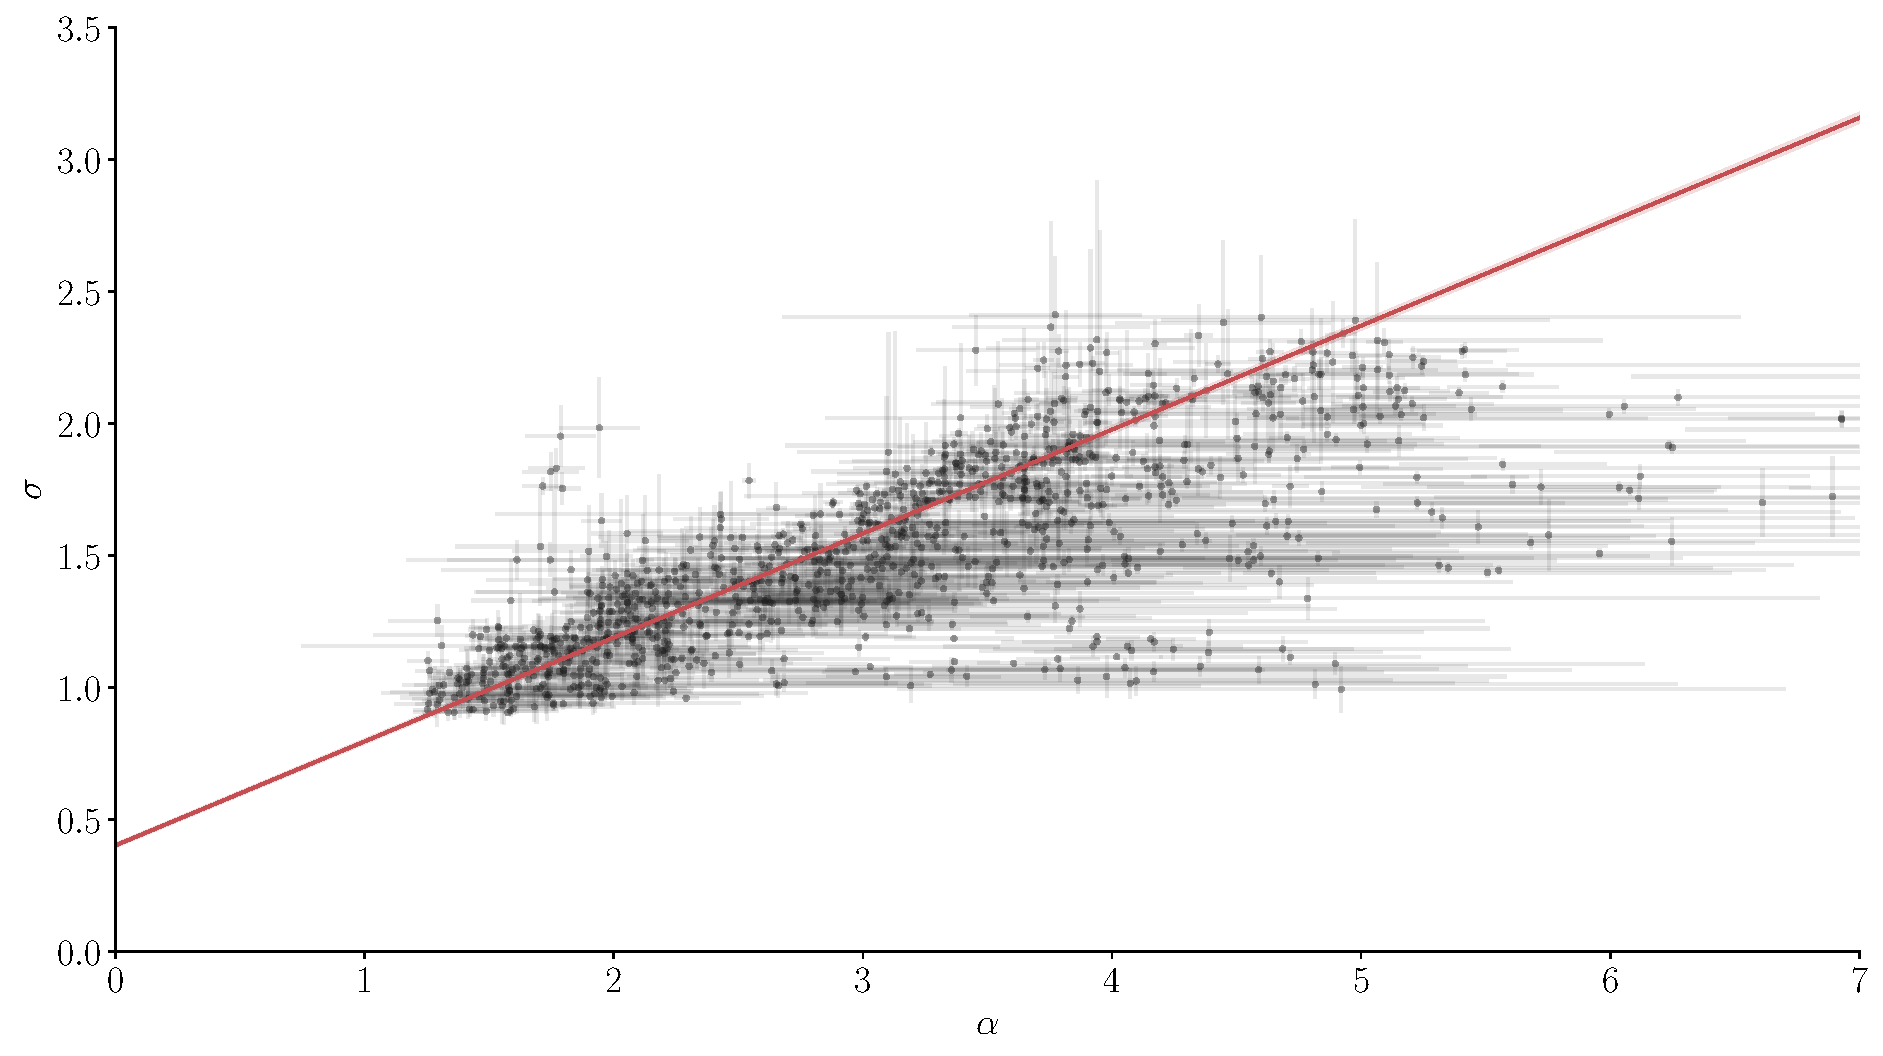
\includegraphics[width=0.8\textwidth]{../figures/06_irf/STD_correlation_betafixed.pdf}
  \caption[]{}
  \label{fig:corralphasigma_achrom}
\end{figure}



\begin{figure}[ht]
  \centering
  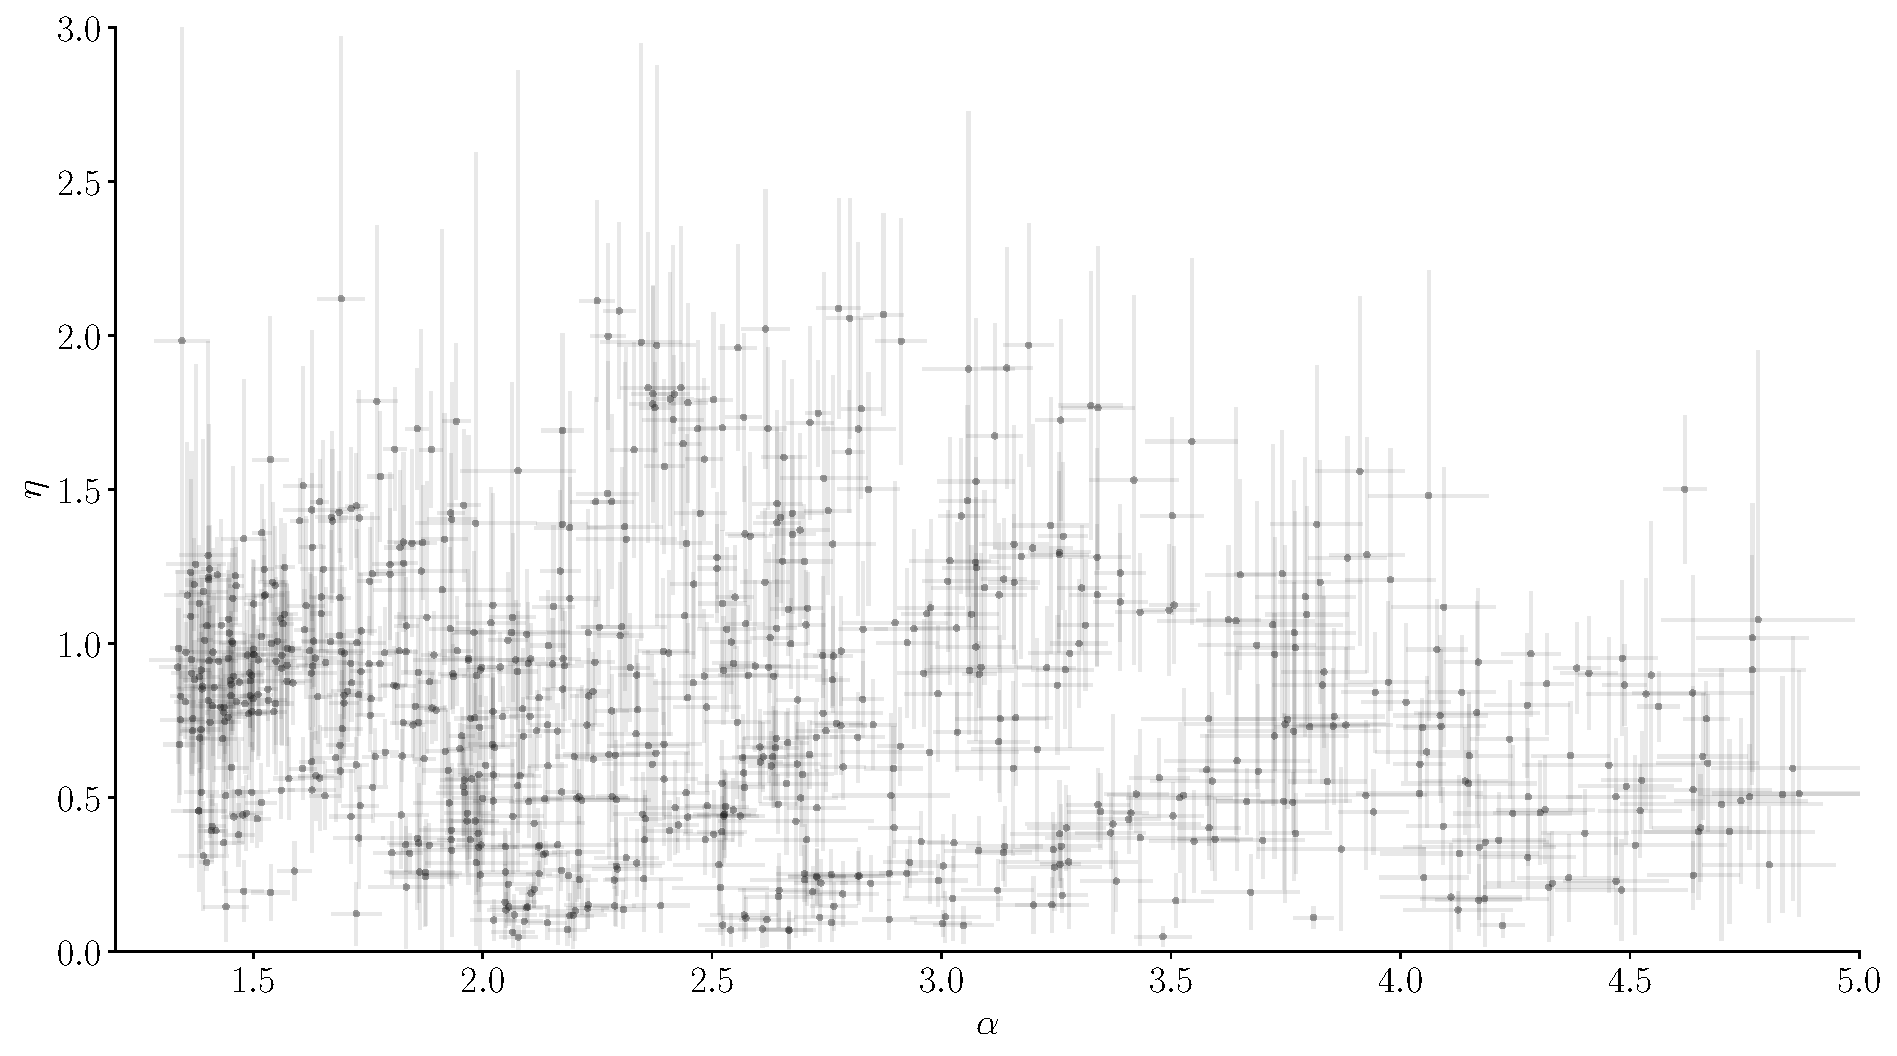
\includegraphics[width=0.8\textwidth]{../figures/06_irf/STD_correlation_betasigmafixed.pdf}
  \caption[]{}
  \label{fig:}
\end{figure}



\begin{figure}[ht]
  \centering
  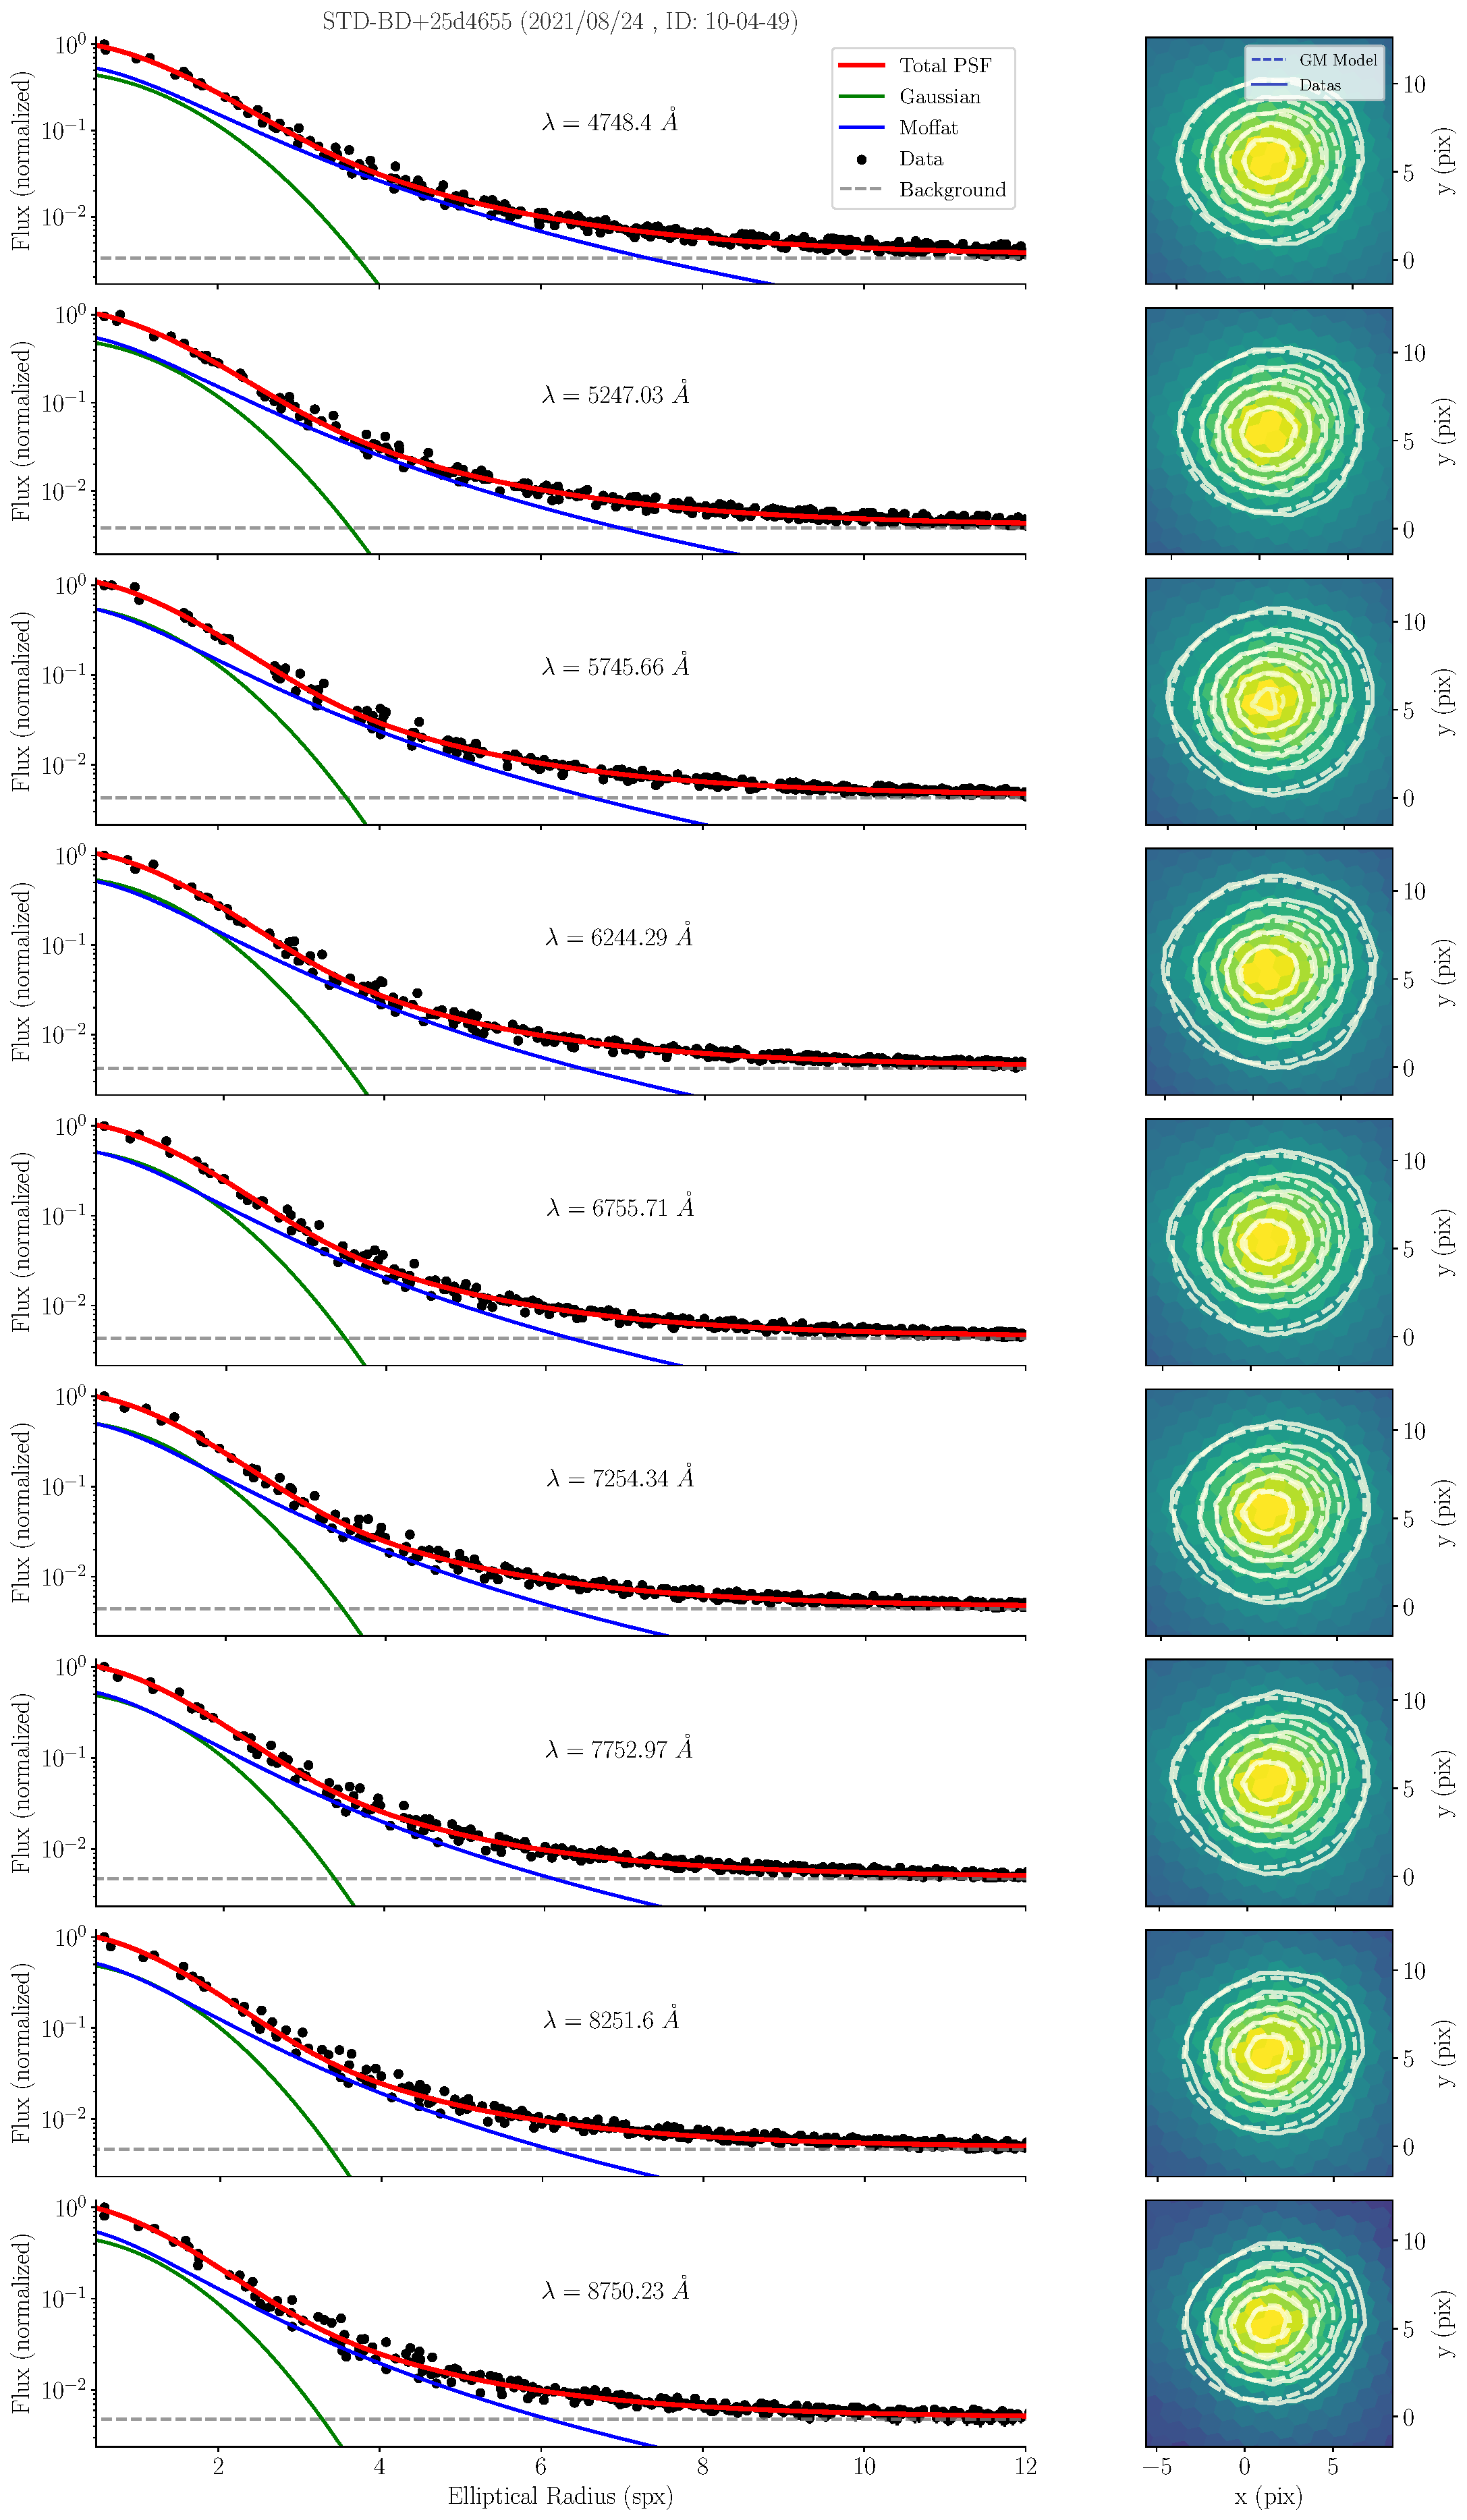
\includegraphics[width=0.7\textwidth]{../figures/06_irf/STD_profile_allmeta.pdf}
  \caption[]{Profil radial et coutours des $9$ metaslices de la STD}
  \label{fig:}
\end{figure}

\subsection{Chromaticité et ADR}\label{ssec:chromadr}

\section{Validation}\label{sec:validationpsf}

\subsection{Calibration photométrique}\label{ssec:photocalibstd}

\subsection{Résultats}\label{ssec:resultscalib}


\bibliographystyle{../main/aa_url2}
\bibliography{99_references}


\message{ !name(06_irf.tex) !offset(529) }

\end{document}

%%% Local Variables:
%%% mode: latex
%%% TeX-master: t
%%% End:
